%--------------------
% Packages
% -------------------
\documentclass[12pt,a4paper]{article}

\input{my-bib-file/usepackage.tex} 

\usepackage{framed}

\title{ \begin{framed} Quantum Information Theory - 67749 \\ 
Recitation 3, \today \end{framed}  }
%\date{\today}
\date{\vspace{-5ex}}


\addbibresource{my-bib-file/sample.bib} 

\begin{document}

\input{my-bib-file/newcommands.tex} 
%\begin{framed}
\maketitle{ }    
%\end{framed}



\newcommand{\CCZ}{\textbf{CCZ}}
\newcommand{\CCX}{\textbf{CCX}}


\newcounter{enumcirc}
\setcounter{enumcirc}{1} 
\counterwithin{enumcirc}{section}


\newcommand{\advanceday}[1][21]{%
\begingroup
\AdvanceDate[#1]%
\today%
\endgroup
}%


\newcommand{\subqCircEx}[2]{\begin{subfigure}[t]{0.5\textwidth}
        \stepcounter{enumcirc} \caption*{ (\alph{enumcirc}) #1} \centering 
        #2
    \end{subfigure}
}

\newcommand{\qCircEx}[4]{\begin{figure*}[h!]
    \centering
    \subqCircEx{#1}{#2}
    ~ 
    \subqCircEx{#3}{#4}
\end{figure*}
}

\newcommand{\qCircExfullline}[2]{\begin{figure*}[h!]
    \stepcounter{enumcirc} \caption*{ (\alph{enumcirc}) #1}
        \centering 
        #2
\end{figure*}
}

\section{Recitation Overview - Quantum Error Correction Codes.}


In the last lectures, we introduced quantum channels - physical maps between density matrices and mentioned that they are used to represent noise, an error that might occur during either computation or communication. Faults and errors are not unique to the quantum regime and were studied before in the context of (classical) error correction codes and fault tolerance. In this recitation, we are first going to represent what classical error correction codes are, and we will give the Tanner codes as an example of the construction of such codes. Then we will talk about the standard way to model quantum noise, give a basic example of a first quantum code, and then eventually we will give the Toric code.

\newcommand{\cH}{\mathcal{H}}
\newcommand{\ketbra}[1]{\ket{#1}\bra{#1}}
\newcommand{\brakett}[3]{\braket{#1 | #2 | #3}}
\newcommand{\old}[1]{}
\newcommand{\tT}{\tilde{T}}
\newcommand{\trace}{ \mathbf{Tr} }




\part{Classicl Error Correction Code.}

  \section{Codes in General. Notations and Definitions.}
  
  A code is a subset, which one can think of as the valid points. Here we focus only on linear binary codes, which are linear subspaces of $\mathbb{F}_{2}^{n}$. Requiring linearity allows us to talk about efficiency. Now, our subspace is the image of the encoding matrix or the kernel of the checking matrix.
  As implied at the beginning, codes are used to correct errors, a correctable error is one that gets a valid point into its local environment. A common way to measure resilience is to ask how many bits an evil entity needs to flip such that the corrupted vector will be closer to another vector in that space than the original one. Those ideas were formulated by Hamming \cite{Hamming}, who presented the following definitions. 
  \begin{definition} \label{bi-code} Let $n \in \mathbb{N}$ and $\rho, \delta\in \left( 0,1 \right)$. We say that $C$ is a \textbf{binary linear code} with parameters $[n, \rho n, \delta n]$. If $C$ is a subspace of $\mathbb{F}_{2}^{n}$, and the dimension of $C$ is at least $\rho n$. In addition, we call the vectors belong to $C$ \textit{codewords} and define the distance of $C$ to be the minimal number of different bits between any codewords pair of $C$.

    
Moreover, since $C$ is a linear subspace, there are matrices $G : \mathbb{F}_{2}^{\rho n} \rightarrow \mathbb{F}_{2}^{n}$ and $H : \mathbb{F}_{2}^{n} \rightarrow \mathbb{F}_{2}^{s}$ such that $C = \image G$ and $C = \ker H$. $G$ is called the generator matrix of $C$, while $H$ is called the parity check matrix of $C$.
  \end{definition}
  From now on, we will use the term code to refer to linear binary codes, as we don't deal with any other types of codes. Also, even though it is customary to use the above parameters to analyze codes, we will use their percent forms called the relative distance and the rate of code, matching $\delta$ and $\rho$ correspondingly.     
  \begin{definition} \label{family} A \textbf{family of codes} is an infinite series of codes. Additionally, suppose the rates and relative distances converge into constant values $\rho,\delta$. In that case, we abuse the notation and call that family of codes a code with $[n, \rho n, \delta n]$ for fixed $\rho, \delta\in [ 0,1 )$, and infinite integers $n \in \mathbb{N}$.     
  \end{definition}
  Notice that the above definition contains codes with parameters attending to zero. From a practical view, it means that either we send too many bits, more than a constant amount, on each bit in the original message. Or that for big enough $n$, adversarial, limited to changing only a constant fraction of the bits, could disrupt the transmission. That distinction raises the definition of good codes.

  \begin{definition} \label{good-code} We will say that a family of codes is a \textbf{good code} if its parameters converge into positive values. 
  \end{definition}


  \begin{example}[The Check-sum/Even-parity Code.]
The parity check code $C_{p} \subset \mathbb{F}_{2}^{n+1}$ consists of codewords that are vectors with even parity. Alternatively, it can be described as appending the xor of the original codeword at the end, sometimes called a checksum bit.
\begin{equation*}
  \begin{split}
    101 &\mapsto 101 \inb{0} \\ 
    111 & \mapsto 111 \inb{1}\\
    000 & \mapsto 000 \inb{0}
  \end{split}
\end{equation*}
  \end{example}

  \begin{example}[The Repetition Code.]  
    Define the repetition code $C_{r} \subset \mathbb{F}_{2}^{n \cdot r}$, In which, for a fixed integer $r$, any bit of the original string is duplicated $r$ times. For example:
\begin{equation*}
  \begin{split}
    0 & \mapsto 0\inb{000}\\
    1 & \mapsto 1\inb{111}
  \end{split}
\end{equation*}
  \end{example}

Having both examples in mind, we get a feeling of the behavior of the distance-rate trade-off. To summarize, using a simple construction, one could construct the codes $[r, 1, r]$ and $[r, r-1, 2]$. Each has a single perfect parameter, while the other decays to the worst. That's bring us to present the Singleton Bound.

  Besides being the first bound, Singleton bound demonstrates how one could get results by using relatively simple elementary arguments. It is also engaging to ask why the proof yields a bound that, empirically, seems far from being tight.
  \begin{theorem*}[Singleton Bound.]\label{theorem*:Sing}  For any linear code with parameter $[n,k,d]$, the following inequality holds:
  \begin{equation*}
    k+ d \le n + 1
  \end{equation*} 
  \end{theorem*}

\begin{proof} Since any two codewords of $C$ differ by at least $d$ coordinates, we know that by ignoring the first $d-1$ coordinate of any vector, we obtain a new code with one-to-one corresponding to the original code. In other words, we have found a new code with the same dimension embedded in $\mathbb{F}_{2}^{n-d+1}$. Combine the fact that dimension is, at most, the dimension of the container space, we get that:  
  \begin{equation*}
    \begin{split}
      \dim C &= 2^{k} \le 2^{n-d+1} \Rightarrow k+d \le n + 1
    \end{split}
  \end{equation*}
\end{proof}

It is also well known that the only binary codes that reach the bound are: $[n,1,n]$, $[n,n-1,2]$,$[n,n,1]$ \cite{eczoo_mds}. In particular, there are no good binary codes that obtain equality(And no binary code which get close to the equality exits). 

Next, we will review Tanner's construction, that in addition to being a critical element to our proof, also serves as an example of how one can construct a code with arbitrary length and positive rate.


Another parameter that will interest us is the complexity of performing checks. Consider a computation model in which the bits are exposed to errors at any time step. In those models, a long check might accumulate faults while being performed. So, if one would like to assume that with non-vanishing probability the check gives a true result, then he has to ensure that it takes constant time.

\begin{definition}[LDPC codes.]
  We will say that a code $C$ is a \textbf{low density parity check matrix} code if any check of it (a row in the parity check matrix), checks toach at most $O(1)$ bits. 
\end{definition}

\begin{exercise}
Give two representations of the checking matrix of the repetition code, one which is LDPC and the other which is not.
\end{exercise}

\section{Tanner Code}
The constructions require two main ingredients: a graph $\Gamma$, and for simplicity, we will restrict ourselves to a $\Delta$ regular graph, Yet notice that the following could be generalize straightforwardly for graphs with degree at most $\Delta$. The second ingredients is a ;small' code $C_{0}$ at length equals the graph's regularity, namely $C_{0} = [\Delta,\rho\Delta, \delta\Delta]$. We can think about any bit string at length $\Delta$ as an assignment over the edges of the graph. Furthermore, for every vertex $v \in \Gamma$, we will call the bit string, which is set on its edges, the local view of $v$. Then we can define, \cite{Tanner}:
  \begin{definition}  Let $ C = \mathcal{T}\left( \Gamma, C_{0} \right)$  be all the codewords which, for any vertex $v\in \Gamma$, the local view of $v$ is a codeword of $C_{0}$. We say that $C$ is a \textbf{Tanner code}\label{Tan} of $\Gamma, C_{0}$. Notice that if $C_{0}$ is a binary linear code, So $C$ is.  
  \end{definition}
  \begin{example}
Consider the Petersen graph $\Gamma$, which is a regular graph with degree $3$. Let $C_{0}$ be the set of all words with even parity. It follows that $C_{0}$ contains all even-length binary strings of length $3$: $000$, $110$, $101$, and $011$. However, the size of $\mathcal{T}(\Gamma, C_{0})$ is significantly larger, as shown in Figure \cref{fig:pet}. Specifically, any rotation of the inner and outer cycles simultaneously gives rise to another valid codeword, so any assignments that are not invariant under these rotations would produce five additional valid codewords.

  \end{example}

  \begin{figure}[h]
    \centering
    \includegraphics[width=\textwidth]{peterson.png}
    \caption{Peterson Graph.}
    \label{fig:pet}
  \end{figure}


%\end{center}
  %It's also worth mentioning that the first construction of good classical codes, due to Sipser and Shpilman, are Tanner codes over expanders graphs \cite{ExpanderCodes}.
  \begin{lemma}
\label{tanrate} Tanner codes have a rate of at least $2\rho - 1$.
\end{lemma}
  \begin{proof}  The dimension of the subspace is bounded by the dimension of the container minus the number of restrictions. So assuming non-degeneration of the small code restrictions, we have that any vertex count exactly $ \left( 1 - \rho  \right)\Delta $ restrictions. Hence, \begin{equation*}
    \begin{split}
      \dim C & \ge \frac{1}{2}n\Delta - \left( 1-\rho \right)\Delta n = \frac{1}{2}n\Delta\left( 2\rho - 1 \right)  
    \end{split}
  \end{equation*} Clearly, any small code with rate $> \frac{1}{2}$ will yield a code with an asymptotically positive rate \end{proof} 
  %\subsubsection{Positive Rate, Arbitrarily Large Codes.} 
  Based on \cref{tanrate}, we can obtain a recipe for constructing codes with a almost non-vanishing rate for arbitrarily large lengths and dimensions. This recipe involves concatenating a series of Tanner codes over complete graphs. To be more precise, we can define a family of codes as follows:
  \begin{equation*}
    \begin{split}
      C_{i+1} & = \mathcal{T}\left( K_{n(C_{i}) + 1}, C_{i} \right) \\
      C_{0} &= \text{ Some simple } \Delta[1, \rho_{0}, \delta_{0}] \text{ code. }
    \end{split}
  \end{equation*}
Where $n(C_i)$ represents the code length of the $i$th code. Repeating the process described above $\log_{\Delta}^{*}(n)$ times allows us to extend the initial code $\Delta[1,\rho_{0}]$ to $n[1, \sim 2\rho^{\log_{\Delta}^{*}(n)}]$. Interestingly, any family of finite groups generated by a constant-size generator set can define a family of codes by utilizing their Cayley graphs as a basis for Tanner codes.

  Once we have seen that Tanner codes enable us to achieve rates, the next natural question to ask is about the distance of the codes. Achieving a linear distance requires a little bit more from the graphs, but to understand this idea better, let us return to the repetition code. For instance, the repetition code can be presented as a Tanner code over the cycle graph.  

  \begin{example}
    In this representation, each vertex checks if the bits on its edges are equal. A valid codeword is an assignment in which all the bits are equal, since otherwise, there would be an edge with no supporting vertex. An illustration of a legal assignment is provided in \cref{fig:cyc}.
    

Recall that the distance of a linear code is the minimal weight of the non-zero codewords. Consider a codeword $c \in C$ and group the vertices by four sets $V_i$ such that $V_i$ is the set of vertices that see $i \in \{0,1\}^{2}$. Since $c \in C$, we have that $|V_{10}|=|V_{01}| = 0$. Additionally, any vertex in $V_{00}$ is not connected to $V_{11}$, which gives us two possible cases: either all the vertices in $V_{11}$ are isolated, or the graph is not connected. Hence, the distance of the code is equal to $\frac{1}{2}\sum{|V_{i}|\cdot |i|} = \frac{1}{2}2 \cdot n = n$.
  \end{example} 


 \begin{figure}[h]
   \begin{center}
  \label{fig:cyc}
\input{~/workspace/Academic/projects/NLTES_project/ltc_ldpc/network2-cycle.tex} 
\caption{The $1^{n}$ assignment on the cycle graph. Any vertex compute parity $1 + 1 = 0$, therefore all the restrictions are satisfied and $1^n \in \mathcal{T} \left( \text{ cycle } , \text{ parity }  \right) $.}
\end{center}
\end{figure}

It is worth mentioning that, in the literature, the repetition code is not usually given as an example of a Tanner code. However, this example will come up again later in the chapter on quantum codes, when we discuss the Toric code, its relation to the hyperproduct code, and how it can be seen as a hyperproduct of two cycle codes.

Furthermore, analyzing the repetition code gives a clue as to how, in certain cases, one might prove a lower bound on the code distance. We would like to say that, if the weight of the code word is below the distance, then it must be that there is at least one vertex that has a non-trivial local view which is not a codeword in $C_{0}$. Put differently, we cannot spread a small weight codeword over $\{V_{i}\}$, defined above, without expanding into subsets corresponding to low $|i|$. Next, we are going to present the Expander codes, which are Tanner codes constructed from graphs with good algebraic expansion.
%Note that for any $S\subset V$ and $ S \neq V $, 

%But on the other hand any vertex in $V_{00}$ can't be connected to $V_{11}$, Thus we obtain that either all the vertices in $V_{11}$ tr that the graph is not connected. The distance of the code is $\frac{1}{2}\sum{|V_{i}|\cdot |i|} = \frac{1}{2}2 \cdot n = n$.      
% The idea  


\part{Quantum Error Correction Codes.}
\section{Introduction.}

The second difference, which is a subtle point, is that quantum states are susceptible to additional types of errors. In addition to the possibility of bit-flip errors, a quantum state may also experience a change in phase. For example, consider the initial state $\ket{+} = \frac{1}{\sqrt{2}}\left( \ket{0} + \ket{1} \right)$, and suppose that due to noise the state is transformed into $\frac{1}{\sqrt{4}}\left( \sqrt{3}\ket{0} + \ket{1} \right)$. Classical circuits are oblivious to such faults, meaning that their operation would remain unchanged as no error has occurred. Quantum circuits, however, are usually affected and may fail. Furthermore, when designing a decoder for quantum error correction codes, one must ensure that the decoding process does not introduce bit-flip errors if a classical code is used to protect against phase flips.

\input{~/workspace/Academic/projects/master-thesis/qnoise.tex} 


Let's return to the repetition code presented in Chapter 2. We would like to have an analog; a first and natural attempt might consider duplicating copies of the state. Unfortunately, copying a general state is not a linear operation and therefore cannot be done in the circuit model (or any other believed to be feasible). In particular, there is no circuit $U$ which can simultaneously duplicate the states $\ket{0}, \ket{1}, \ket{+}, \ket{-}$.

To overcome the issue, Shor came up with the nine-qubit code \cite{Ninequ}, which at first glance might seem a naive straightforward implementation of ``duplication'', but instead uses a clever insight about quantumness in general. Any operation can be seen as a linear (and even unitary) operation over a subspace embedded in a large enough dimension. The encoding is given as follows: 
\begin{equation*}
  \begin{split}
    |\overline{0}\rangle&=\frac{1}{2\sqrt{2}}\left(|000\rangle+|111\rangle\right)^{\otimes3}\\
    |\overline{1}\rangle&=\frac{1}{2\sqrt{2}}\left(|000\rangle-|111\rangle\right)^{\otimes3}~.
  \end{split}
\end{equation*}


For convenience, let us use the notation $\ket{\mathbf{GHZ}^{\pm}} =  \ket{0^{m}} \pm  \ket{1^{m}}$. We can also consider the Shor code over $m^{2}$ qubits, which is defined as above, such that any logical state contains $m$ products over $m$ qubits. Therefore, the state $\ket{\overline{0}}$ over $m^{2}$ qubits can be written as $\ket{\mathbf{GHZ}^{+}}^{m}$. We are now ready to prove a statement regarding the robustness.
\begin{lemma}
  The Shor code over $9$ qubits enable to correct a single either bit or phase flip.  
\end{lemma}
It is evident that a single bit-flip error can be handled in the same way as in the conventional case. The decoder will check if any of the triples have the same value, and if not, it will correct it by majority. To create a decoder that can also correct a phase-flip error, we need the following statement. In this chapter, we denote the Hadamard gate over $m$ qubits as $H^m$.
\begin{claim}
   $H^{m}\ket{\mathbf{GHZ}^{\pm}} = \sum_{ x \cdot \mathbf{1} =_2 \pm }{\ket{x} }$
\end{claim}

\begin{proof}

  \begin{equation*}
    \begin{split}
      H^{m}\ket{\mathbf{GHZ}^{\pm}} & = H^{m}\ket{0^{m}} \pm  H^{m}\ket{1^{m}} = \sum_{x \in \mathbb{F}_{2}^{m}}{\ket{x}} \pm  \sum_{x \in \mathbb{F}_{2}^{m}}{\left( -1 \right)^{x \cdot \mathbf{1}} \ket{x}} \\ & = \sum_{x \in \mathbb{F}_{2}^{m}}{ \left( 1 \pm \left( -1 \right)^{x \cdot \mathbf{1}}  \right) \ket{x} } =  \sum_{x \cdot \mathbf{1} =_2 \pm }{\ket{x} }
    \end{split}
  \end{equation*}
\end{proof}

Now it is clear how to correct a phase flip. One can apply the Hadamard transform and compute the parity of each triple. By the assumption that only a single phase flip may occur, either all the triples have the same parity or the faulted one has an opposite parity and needs to be corrected. Thus, we obtain an $\left[ \left[ 9,1,3 \right] \right]$ quantum error correction code. Asymptotically, this is an $\left[ \left[ m^{2}, 1, m \right] \right]$ code.

\section{CSS Codes.}

The Shor code is a specific case of the more general CSS (Calderbank-Shor-Steane) code \cite{Calderbank_1996}. A family composed by two binary codes $C_{X}, C_{Z}$ such that $C_{Z}^{\perp} \subset C_{X}$. 

\input{~/workspace/Academic/projects/master-thesis/css.tex}

  \section{qLDPC Codes.}
  As exactly as in the classic case, qLDPC codes are codes in which any check act non trivially on at most a constant number of qubits, It was proved that using a good Quantum LDPC code one can achieve a fault tolerance threshold theorem at the cost of only constant overhead\footnote{under the assumption of having an efficient decoder.} \cite{gottesman2014faulttolerant}. We are now about to embark on a detailed review of the first quantum LDPC code \cite{Dennis_2002}. 

  Recall that one way to present a code is by define the parity check matrix, Consider the $l\times l$ Tours, namely the Cayley graph of the group product  $\mathbb{Z}_{l} \times \mathbb{Z}_{l}$. Associate any coordinate (bit/qubit) with an edge on the Tours. And consider the following two restrictions:

  \begin{enumerate}
    \item Each vertex requires form its local view, the bits lay on its supported edges, To has an even party. We will refer to this type of check as \textit{cross check}. Namely $C_{X}$ is the tanner code defined by use the Toric as a graph and the parity code as the local code. 
    \item Similarly, each face requires the same from its supported edges but computes the parity in a phase basis, namely the $C_{Z}$ code defined again as Tanner code, when the graph is defined by associating with each face a vertex and connecting any two adjacent faces by an edge, which corresponds to the side of the square.
  \end{enumerate}

  \begin{center}
    \begin{figure}[H]
  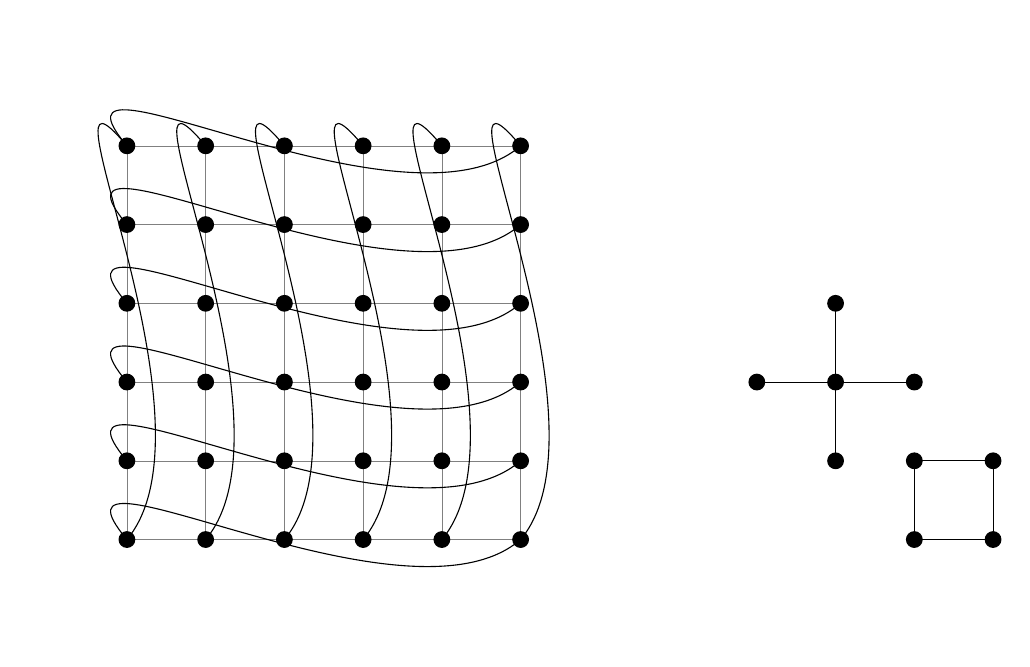
\begin{tikzpicture}
  \draw[step=1cm,gray,very thin] (0,0) grid (5,5);
  \foreach \x in {0,1,2,3,4,5}
  \foreach \y in {0,1,2,3,4,5}
  {
  \node[draw,circle,inner sep=2pt,fill] at (\x,\y) {};
}
\draw[ -> ]  (0,0) to [out=50, in=130] (0,5);
\draw[ -> ]  (1,0) to [out=50, in=130] (1,5);
\draw[ -> ]  (2,0) to [out=50, in=130] (2,5);
\draw[ -> ]  (3,0) to [out=50, in=130] (3,5);
\draw[ -> ]  (4,0) to [out=50, in=130] (4,5);
\draw[ -> ]  (5,0) to [out=50, in=130] (5,5);
\draw[ -> ]  (0,5) to [out=130, in=220] (5,5);
\draw[ -> ]  (0,4) to [out=130, in=220] (5,4);
\draw[ -> ]  (0,3) to [out=130, in=220] (5,3);
\draw[ -> ]  (0,2) to [out=130, in=220] (5,2);
\draw[ -> ]  (0,1) to [out=130, in=220] (5,1);
\draw[ -> ]  (0,0) to [out=130, in=220] (5,0);

\node[draw,circle,inner sep=2pt,fill] at (9,2) {};
\node[draw,circle,inner sep=2pt,fill] at (10,2) {};
\node[draw,circle,inner sep=2pt,fill] at (8,2) {};
\node[draw,circle,inner sep=2pt,fill] at (9,1) {};
\node[draw,circle,inner sep=2pt,fill] at (9,3) {};
\draw[ -> ]  (9,2) to (10,2);
\draw[ -> ]  (9,2) to (8,2);
\draw[ -> ]  (9,2) to (9,1);
\draw[ -> ]  (9,2) to (9,3);
%\draw[ -> ]  (9,2) to (5,0);

\node[draw,circle,inner sep=2pt,fill] at (10,1) {};
\node[draw,circle,inner sep=2pt,fill] at (11,1) {};
\node[draw,circle,inner sep=2pt,fill] at (10,0) {};
\node[draw,circle,inner sep=2pt,fill] at (11,0) {};
\draw[ -> ]  (10,1) to (11,1);
\draw[ -> ]  (10,1) to (10,0);
\draw[ -> ]  (10,0) to (11,0);
\draw[ -> ]  (11,1) to (11,0);
\end{tikzpicture}
\caption{On the left is the Toric Graph. On the right are cross and face checks.}
\label{fig:Toric}
\end{figure}
\end{center}
%For example consider some vertex $v$ on the Torus, and let $\ket{\psi} = \sum_{x}{ \ket{\cdots x_{e_0}x_{e_1}x_{e_2}x_{e_3}  \cdots}}$ when $e_{0},e_{1},e_{2},e_{3}$ are the edges compose the local view of $v$. Then in any ket can be in the support of $\ket{\psi}$ only if the parity of $e_{0},e_{1},e_{2},e_{3}$ is even.
%\subsection{Note on the Toric in the presence of noise.} 

\begin{claim}
  The $l \times l$  Toric code is a CSS code, with dimension $2$ and distance $\Theta\left( l \right)$.   
\end{claim}





\printbibliography 


\end{document}

